\chapter{Methods}
\label{chap:methods}

\section{System Overview and Design Rationale}
\label{sec:meth-overview}
% Two decoupled stacks: generation (dialogue creation) and evaluation
%   (stability measurement)
%   Why decoupled? Evaluation must not be contaminated by generation-side
%   randomness -- reproducible entry points require frozen, pre-generated histories
% End-to-end data flow:
%   vignettes -> generation -> frozen histories -> evaluation -> aggregation
% [FIG] Full pipeline diagram -- logical data flow across all stages, stack
%   boundary marked, example artefact names at each step

The evaluation system separates dialogue creation from stability measurement
through two decoupled stacks. The \emph{generation stack} produces synthetic
therapy sessions by running a multi-agent dialogue loop. The
\emph{evaluation stack} measures the stability of therapeutic responses by
presenting frozen conversation histories to the model under test and
collecting multiple independent outputs.

This separation is a deliberate design choice. If the evaluation stack
generated its own dialogue context, any measured instability could reflect
upstream randomness in the patient or routing agents rather than genuine
variation in the therapist model. By freezing the conversation history before
evaluation begins, the system ensures that every trial receives identical
input. Any observed inconsistency is attributable solely to the model under
test.

The end-to-end data flow proceeds in three stages: patient vignettes feed the
generation stack, which produces complete therapy sessions. These sessions
are sliced at rescripting-turn boundaries to create frozen histories. The
evaluation stack presents each frozen history to the therapist model across
multiple independent trials, collecting both a strategy declaration and a
therapeutic response per trial. Finally, an aggregation pipeline aligns all
metrics across conditions for comparative analysis.

\begin{figure}[t]
  \centering
  \hspace*{0.4cm}\makebox[\textwidth]{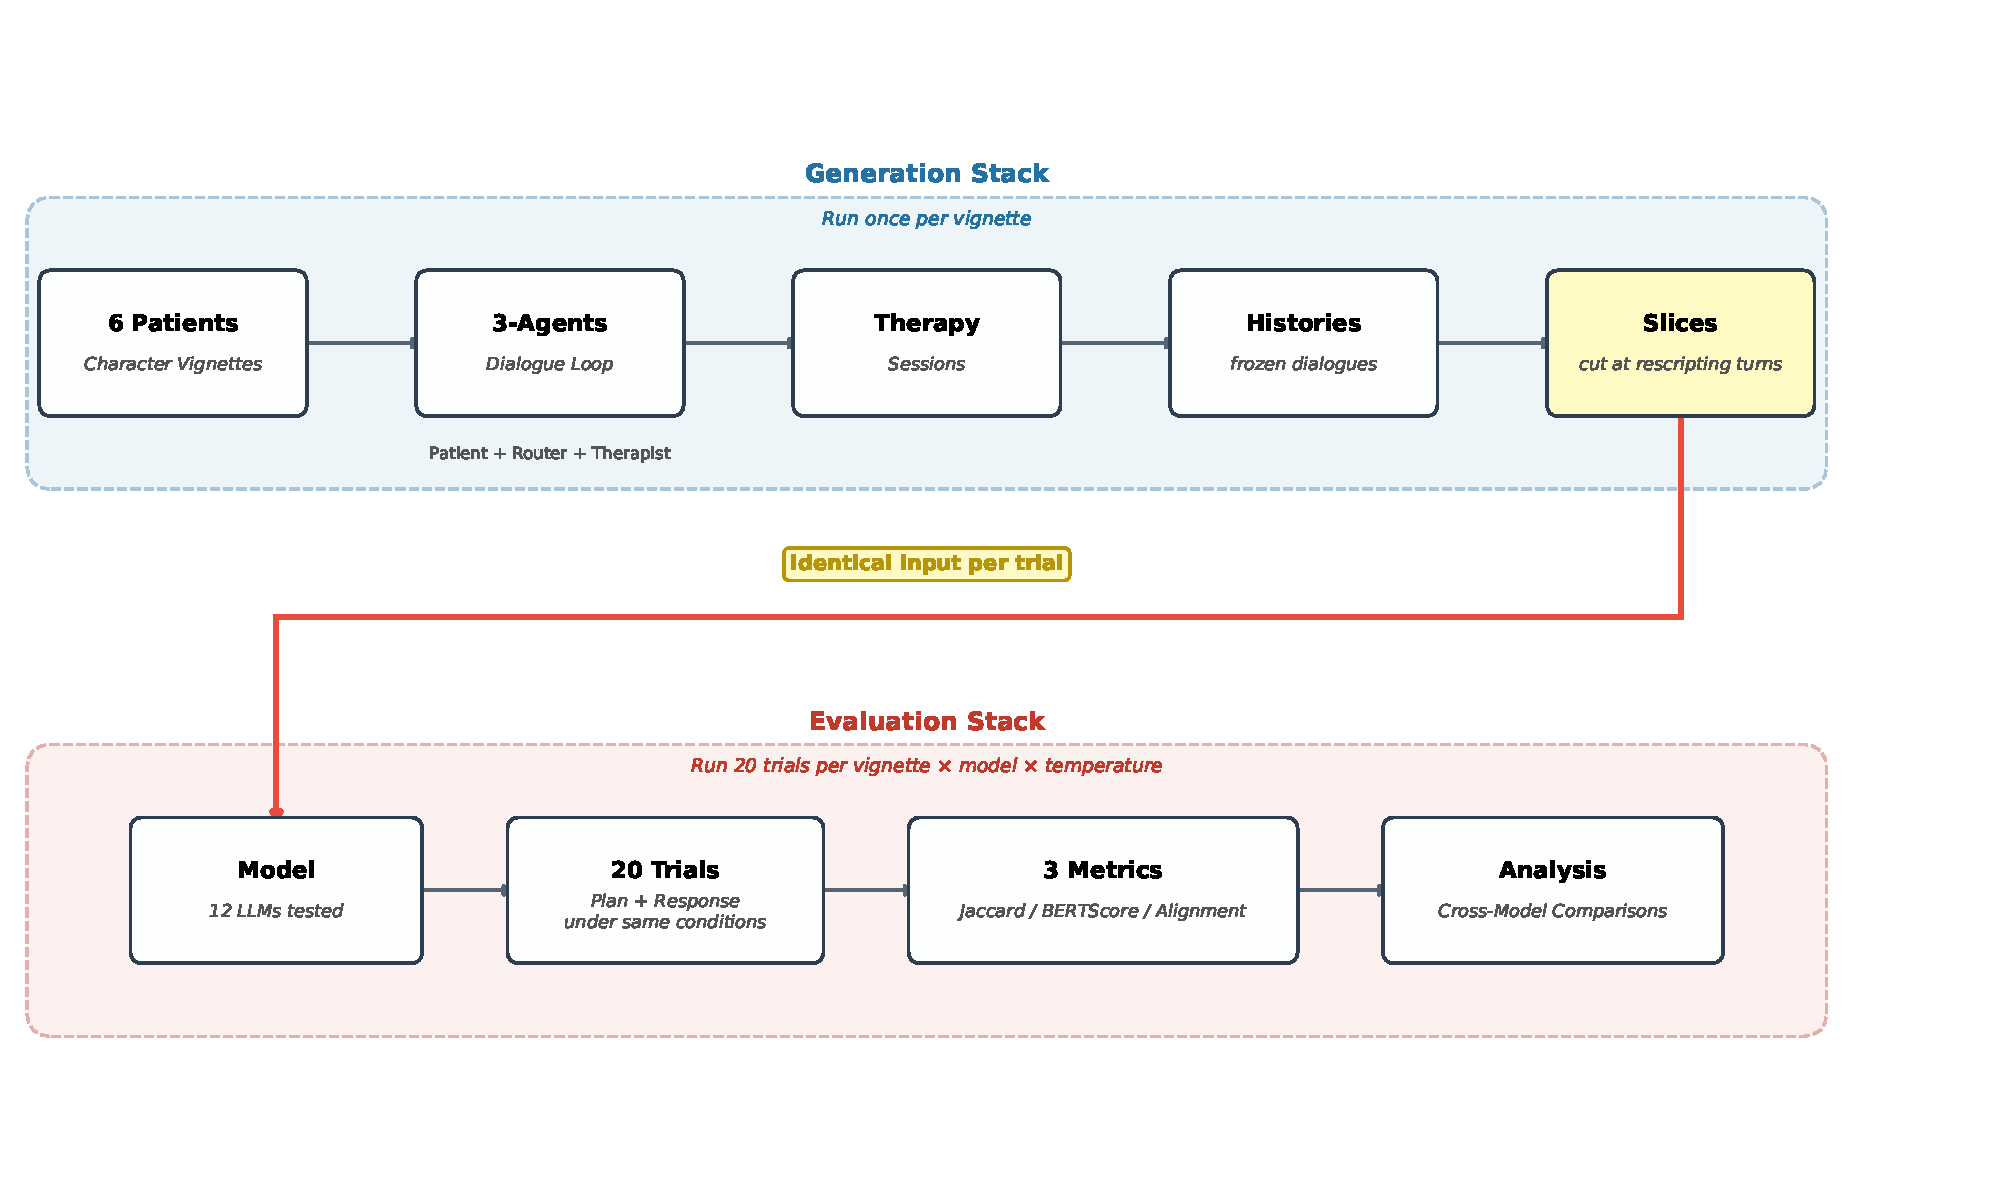
\includegraphics[width=1.2\textwidth]{figures/fig_3_1_pipeline.pdf}}
  \caption{Two-stack pipeline. The generation stack produces frozen
    conversation histories (run once). The evaluation stack presents each
    history to the model under test across twenty independent trials per
    condition. The stacks are decoupled so that evaluation-side variance
    cannot be contaminated by generation-side randomness.}
  \label{fig:pipeline}
\end{figure}


\section{Dialogue Generation}
\label{sec:meth-dialogue}
% Three-agent loop: Patient (BDI-profiled vignette), Router (stage classifier),
%   Therapist (stage-appropriate response)
%   Why three agents? Mirrors clinical interaction structure; separates
%   routing logic from therapeutic content generation
% Six patient vignettes: anxious, avoidant, cooperative, resistant, skeptic, trauma
%   Cover the range of clinical presentation difficulty expected in IRT deployment
%   Vignette design informed by prior synthetic patient work (Roleplay-doh??, check ref).
%   Six profiles sample the difficulty range but do not claim exhaustive coverage (7.2).
% Full three-stage IRT traversal produces naturalistic conversation histories
%   used as frozen evaluation entry points
% [FIG] Three-agent loop -- single turn cycle with message passing
% [Example] Resistant vignette excerpt -- BDI profile and opening patient turn

The generation stack orchestrates a three-agent loop that produces
naturalistic \gls{irt} sessions. Each turn passes through three agents:

\begin{itemize}
  \item \textbf{Patient:} responds based on a behavioural profile
    (nightmare content, emotional style, engagement pattern).
  \item \textbf{Router:} classifies the current protocol stage
    (recording, rescripting, or rehearsal).
  \item \textbf{Therapist:} generates a stage-appropriate response,
    guided by the router's classification.
\end{itemize}

The vignette design is informed by anonymised session data from a prior
reDreamAI efficacy study. Because data protection requirements prevent
using real patient transcripts directly, synthetic patient profiles were
created and validated against published clinical research on simulated
patients.

Six vignettes cover the range of clinical presentation difficulty
expected in \gls{irt} deployment: \emph{anxious}, \emph{avoidant},
\emph{cooperative}, \emph{resistant}, \emph{skeptic}, and \emph{trauma}.
These profiles range from a cooperative patient who engages readily with
rescripting instructions to a trauma patient whose nightmare content
triggers intense emotional responses during the session. The design
draws on prior synthetic patient work. \textcite{Z22JYAMU} demonstrate that
expert-defined behavioural principles produce clinically plausible simulated
patients. \textcite{CQ94GEYA} provide cognitive conceptualisation diagrams
and conversational styles (direct, resistant, expressive, minimal, deviating,
agreeable) that parallel the six profiles used here. Six profiles sample
the difficulty range but do not claim exhaustive coverage of patient
variability (see \autoref{sec:concl-limitations}).

The generation stack traverses the full three-stage \gls{irt} protocol,
producing complete therapy sessions that are then sliced to create
evaluation entry points. \autoref{fig:dialogue-gen} illustrates this
process: the dialogue loops through recording and rescripting until each
stage is complete, then proceeds to rehearsal. Frozen history slices are
cut from the rescripting stage.

\begin{figure}[t]
  \centering
  
\includegraphics[width=\textwidth]{figures/dialogue_generation.png}
  \caption{Dialogue generation loop. The three-agent system traverses
    recording, rescripting, and rehearsal. Frozen history slices for the
    experiment are cut at rescripting-turn boundaries.}
  \label{fig:dialogue-gen}
\end{figure}

% [Example] Resistant vignette excerpt -- BDI profile and opening turn


\section{Frozen History Design}
\label{sec:meth-frozen}
% Deterministic evaluation entry points: identical context for every trial
% Conversations sliced at rescripting-turn boundaries
%   Why frozen? Any measured inconsistency is attributable solely to the
%   model under evaluation -- not to upstream context differences
% Slice depth pilot: 5 depths tested on Mistral Large 3 to select evaluation point
%   Slice 1: introduction to rescripting, moderate variability
%   Slice 2: lowest consistency -- strategy not yet anchored (conservative choice)
%   Slices 3-5: strategy locks in, consistency rises to ceiling
% Main experiment runs at slice 2 (mid-rescripting) -- conservative lower bound
% [FIG] Slicing diagram -- P/T turn sequence with cut points; which turns are
%   in-context vs. excluded per slice

Frozen conversation histories serve as deterministic evaluation entry
points. Each vignette's complete therapy session is sliced at
rescripting-turn boundaries, where each slice ends after a complete
therapist-patient exchange. Every trial, across all models and
temperatures, receives the identical frozen history as input. This design
eliminates context variation as a confound: if two trials produce different
therapeutic responses, the difference is attributable to the model's
stochastic sampling, not to differences in the input conversation.

A preliminary analysis tested \modelname{Mistral Large~3} at five slice
depths across all six vignettes at $T = 0.075$ and $T = 0.15$. Jaccard
consistency was lowest at the second slice (mean $J = 0.77$ at $T = 0.075$)
and rose to near-ceiling values from the third slice onward ($J > 0.93$).
The main experiment evaluates at the second rescripting-turn boundary
(\techil{slice\_2}), making the measured stability a conservative estimate.
Slice depth effects are reported in \autoref{sec:res-secondary}.

% [FIG] Slicing diagram -- P/T turn sequence with slice 2 marked


\section{Evaluation Stack}
\label{sec:meth-eval}
% Router bypassed -- rescripting prompt injected directly (stage known a priori)
%   Why bypass? Isolates the therapist model from stage-classification error
% Fused CoT generation: <plan> block + response in a single model call
%   <plan> block declares 1-2 strategies before the therapeutic response
%   Plan conditions the response tokens (Chain-of-Thought style)
%   Why fused? Plan must condition the response tokens -- a separate call
%   would decouple intent from output
% 20 independent trials per condition sample the stochastic output distribution
% [FIG] Evaluation stack -- frozen history -> injected prompt -> fused generation
% [Example] Raw model output: <plan> block and response side by side

The evaluation stack bypasses the router and injects the rescripting prompt
directly into the therapist model. Because the \gls{irt} stage is known a
priori (all frozen histories are sliced within the rescripting phase), routing
is unnecessary and would introduce an additional source of variation.
Bypassing it isolates the therapist model from stage-classification error.

Each evaluation trial uses \emph{fused generation}: the model produces a
\techil{<plan>} block declaring one to two therapeutic strategies, followed
by the therapeutic response, in a single call. The plan tokens condition the
response tokens in a \gls{cot}-style generation, so the response is
directly conditioned on the declared strategy. This fused approach enables
the coherence analysis in Method~3 (\autoref{sec:meth-m3}): because plan
and response are generated in a single pass, any mismatch between declared
intent and executed strategy reflects the model's own inconsistency rather
than a decoupling artefact. \autoref{fig:eval-stack} illustrates this
measurement design.

\begin{figure}[t]
  \centering
  \makebox[\textwidth]{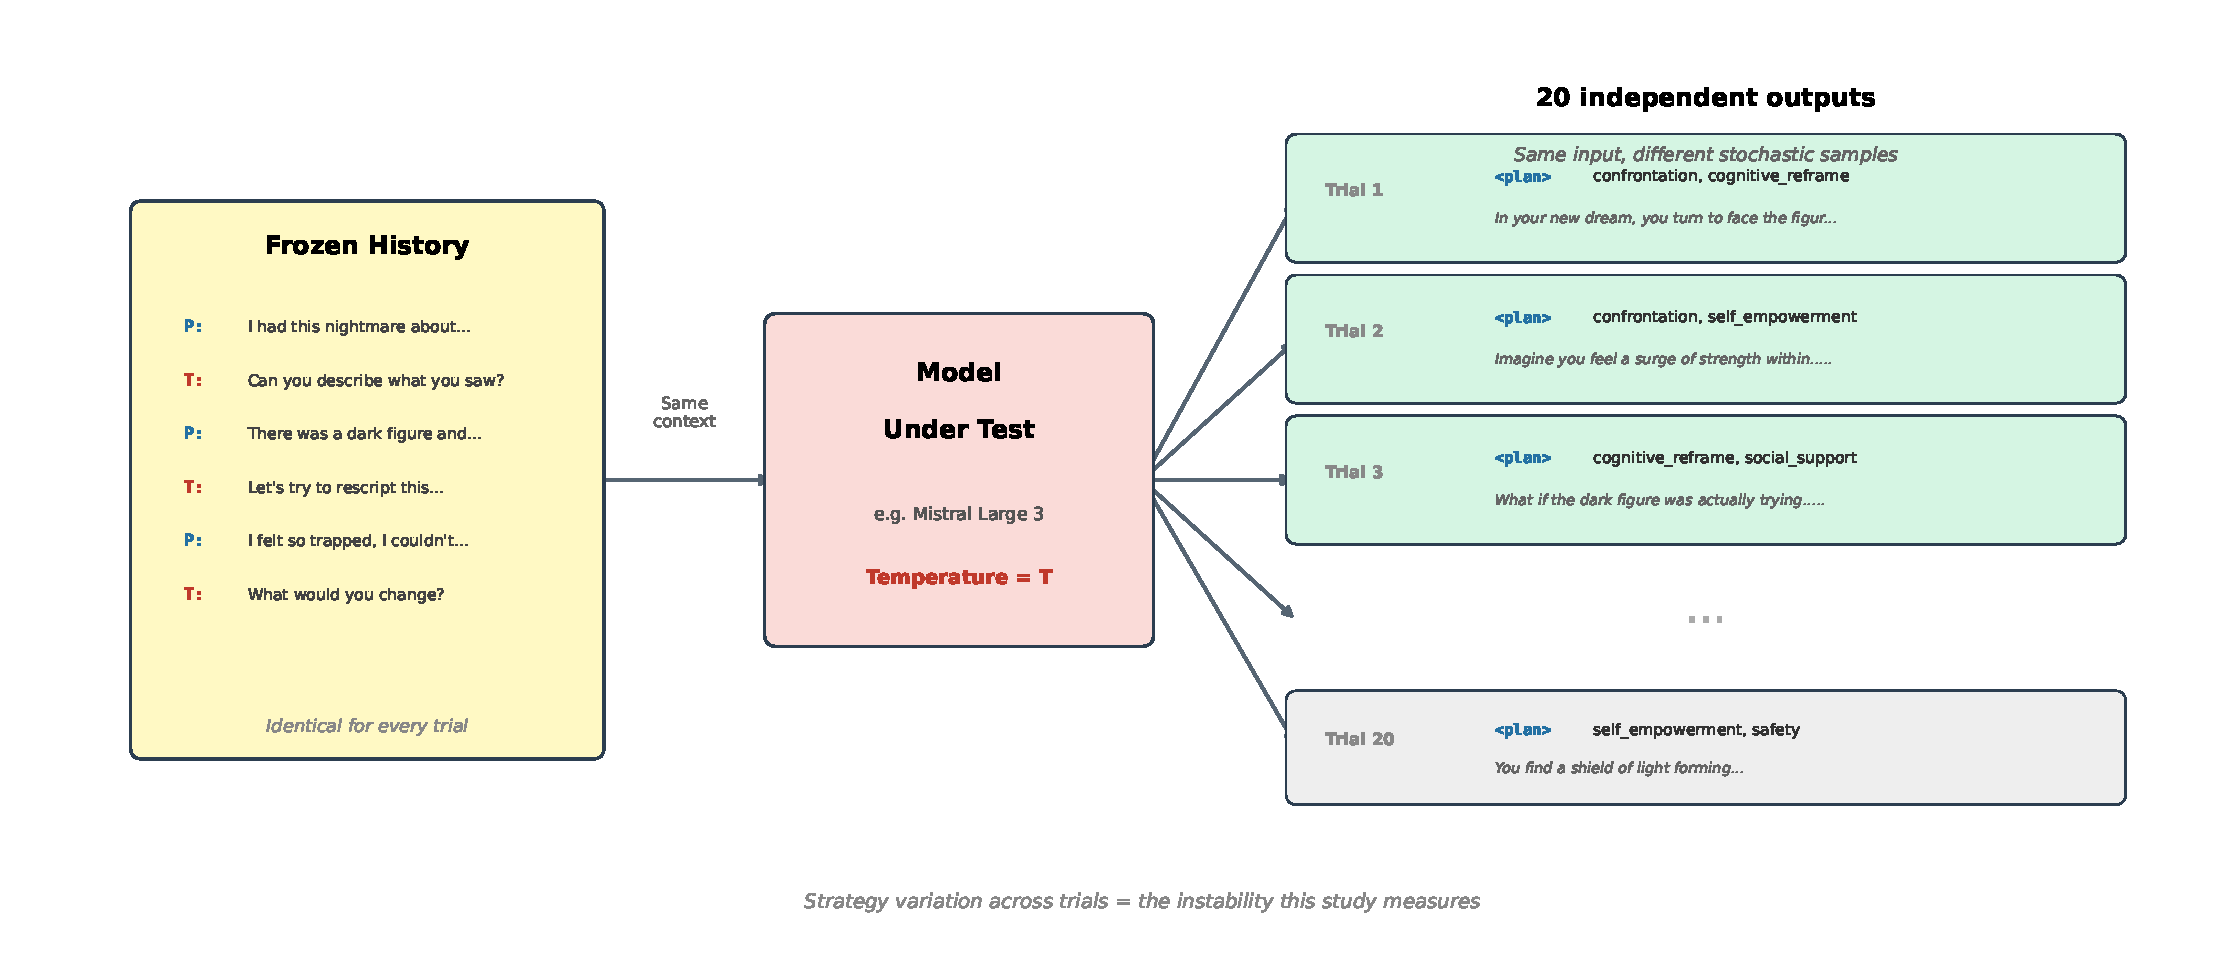
\includegraphics[width=1.1\textwidth]{figures/fig_3_3_eval_stack.pdf}}
  \caption{Measurement design. The same frozen history is presented to
    the model under test twenty times. Each trial independently produces
    a plan and a therapeutic response. Variation across trials is the
    instability this study measures.}
  \label{fig:eval-stack}
\end{figure}

Twenty independent trials are collected per condition, yielding
$\binom{20}{2} = 190$ pairwise comparisons. This trial count balances
statistical power with compute cost: 190 pairs provide robust coverage
of the pairwise similarity distribution while keeping the total experiment
within budget.

% [FIG] Evaluation stack -- frozen history, injected prompt, fused output
% [Example] Raw model output: <plan> block and response side by side


\section{The Plan Mechanism}
\label{sec:meth-plan}
% The CoT faithfulness problem (folded from Background):
%   CoT prompting (Wei et al., 2022) improves output structure, but
%   faithfulness literature (Turpin et al., 2023; Lanham et al., 2023) shows
%   that CoT explanations often do not reflect actual computation. If a model
%   declares its strategy before responding, that declaration may be post-hoc
%   rationalization rather than a window into its decision-making.
%
% Resolution: <plan> block declares 1-2 IRT strategies before the response
% Framed as declared intent -- a structured output, not a reasoning trace
%   Why? Sidesteps the CoT faithfulness problem: the plan is not claimed to
%   be a window into model cognition. It is a measurable output in its own right.
%   If strategy declarations vary across runs, clinical responses will vary --
%   this is true regardless of whether declarations reflect internal reasoning
% Structured measurement independent of CoT faithfulness debate
% Enables three independent uses:
%   1. Strategy-level consistency scoring (Method 1)
%   2. Plan-response coherence verification (Method 3)
%   3. Human-readable clinical oversight
% Fixed IRT strategy taxonomy constrains declarations to the therapeutic domain --
%   prevents arbitrary strategies that cannot be clinically evaluated
% [FIG] Plan mechanism -- <plan> block feeding into three downstream uses
%   with declared-intent framing labelled

The \techil{<plan>} block raises a methodological question. The
faithfulness literature shows that \gls{cot} explanations do not always
reflect a model's actual computation \parencite{TMCBKEVQ, W4K3ARI5}. A
declared therapeutic strategy may therefore be a post-hoc rationalisation
rather than a window into the model's decision-making. This study
sidesteps the problem by framing the plan as \emph{declared intent}: the
plan captures what the model commits to, not what it internally computes.
Whether or not the declaration reflects genuine reasoning, a practical
consequence holds: if strategy declarations vary across runs, clinical
responses will also vary.

This framing sidesteps the faithfulness debate entirely while preserving
three uses. First, the declared strategies enable consistency scoring
on strategy level (Method~1, \autoref{sec:meth-m1}). Second, comparison
between declared strategies and the executed response enables coherence
verification (Method~3, \autoref{sec:meth-m3}). Third, the plan provides
a human-readable summary of the model's intended approach, supporting
clinical oversight in deployment.

% [FIG] Plan mechanism -- <plan> block feeding into three downstream uses


\section{Strategy Taxonomy Development}
\label{sec:meth-taxonomy}
% Why fixed? Enables discrete, comparable strategy sets -- free-text plans
%   cannot be aggregated into Jaccard similarity scores
% Iterative revision driven by observed distribution failures:
%   v1 (8 categories): 87.7% mass on empowerment/mastery -> unusable skew
%   v2 (merge to agency): 100% dominance -> goal-mechanism conflation
%   v3 (mechanism-specific split): confrontation (external action) vs.
%     self_empowerment (internal transformation)
% Final 6 categories: confrontation, self_empowerment, safety, cognitive_reframe,
%   social_support, sensory_modulation
% Prompt-level steering encourages diversity across categories
% [GRAPH] Strategy frequency per taxonomy version (v1 -> v3) -- shows skew
%   collapse and final distribution
% [FIG] 6-category taxonomy card -- each category, definition, example phrase

A fixed taxonomy constrains the \techil{<plan>} block to a predefined set
of therapeutic strategies. This constraint is necessary for quantitative
evaluation: free-text plans cannot be aggregated into set-similarity
scores. The taxonomy evolved through four iterations to resolve
distribution skew in early versions (full revision history in
\autoref{app:taxonomy}). The core design principle is that each category
must describe a rescripting \emph{mechanism} rather than a therapeutic
\emph{goal}. Early versions that used goal-level labels (e.g.\
\emph{empowerment}, \emph{mastery}) produced extreme skew because
every rescripting intervention serves the goal of increased mastery.
Splitting categories along the mechanism dimension resolved this.

The final six-category taxonomy (\autoref{tab:taxonomy}) captures
concrete therapeutic mechanisms:

\begin{table}[t]
  \centering
  \caption{Strategy taxonomy (v4). Each category describes a rescripting mechanism rather than a therapeutic goal.}
  \label{tab:taxonomy}
  \begin{tabularx}{\textwidth}{lX}
    \toprule
    Category & Mechanism \\
    \midrule
    \emph{confrontation}      & The dreamer directly faces, fights, or stands up to the threat \\
    \emph{self-empowerment}   & The dreamer gains a new ability or inner strength \\
    \emph{safety}              & A physical barrier, shelter, or protective figure shields the dreamer \\
    \emph{cognitive reframe}  & Existing dream elements change meaning \\
    \emph{social support}     & A new person, companion, or ally is introduced \\
    \emph{sensory modulation} & Sensory qualities shift, including internal somatic calming \\
    \bottomrule
  \end{tabularx}
\end{table}

The six categories operationalise the clinical rescripting strategies
introduced in \autoref{sec:bg-irt}. Avoidance and distancing are
excluded because they do not resolve the nightmare threat.
\textcite{34DFEBDG} review that \gls{irt} works by increasing mastery
over the nightmare, and that avoidance reinforces the fear memory rather
than overwriting it. \textcite{25UR8BHJ} found that distancing was the
least-used strategy (8\%) and that violence in rescripted dreams
predicted worse outcomes. Reality markers fall outside single-turn
rescripting.

Taxonomy design directly shapes measured consistency. A coarse taxonomy
inflates agreement (every trial lands in the same category), a fine one
deflates it. The sensitivity of scores to category boundaries is
revisited in the discussion (\autoref{sec:disc-framework-design}).

% [GRAPH] Strategy frequency per taxonomy version (v1-v4)
% [FIG] 6-category taxonomy card with definitions and example phrases


\section{Evaluation Metrics}
\label{sec:meth-metrics}
% Why three methods? Each targets a distinct layer of the generation process --
%   no single metric captures the full picture of therapeutic stability
%   Method 1 (Plan Consistency): does the model select the same strategies?
%   Method 2 (Response Similarity): does the model produce equivalent responses?
%   Method 3 (Plan-Response Coherence): does the model do what it declared?
% [FIG] Three-level framework -- plan -> output -> alignment; inputs and outputs
%   of each method, with the clinical question each answers

Three evaluation methods target distinct layers of the generation process.
No single metric captures the full picture of therapeutic stability
(\autoref{sec:bg-metrics}). Method~1 asks whether the model makes consistent
therapeutic decisions. Method~2 asks whether it produces consistent
therapeutic responses. Method~3 asks whether it does what it says it will
do.

\begin{figure}[t]
  \centering
  \makebox[\textwidth]{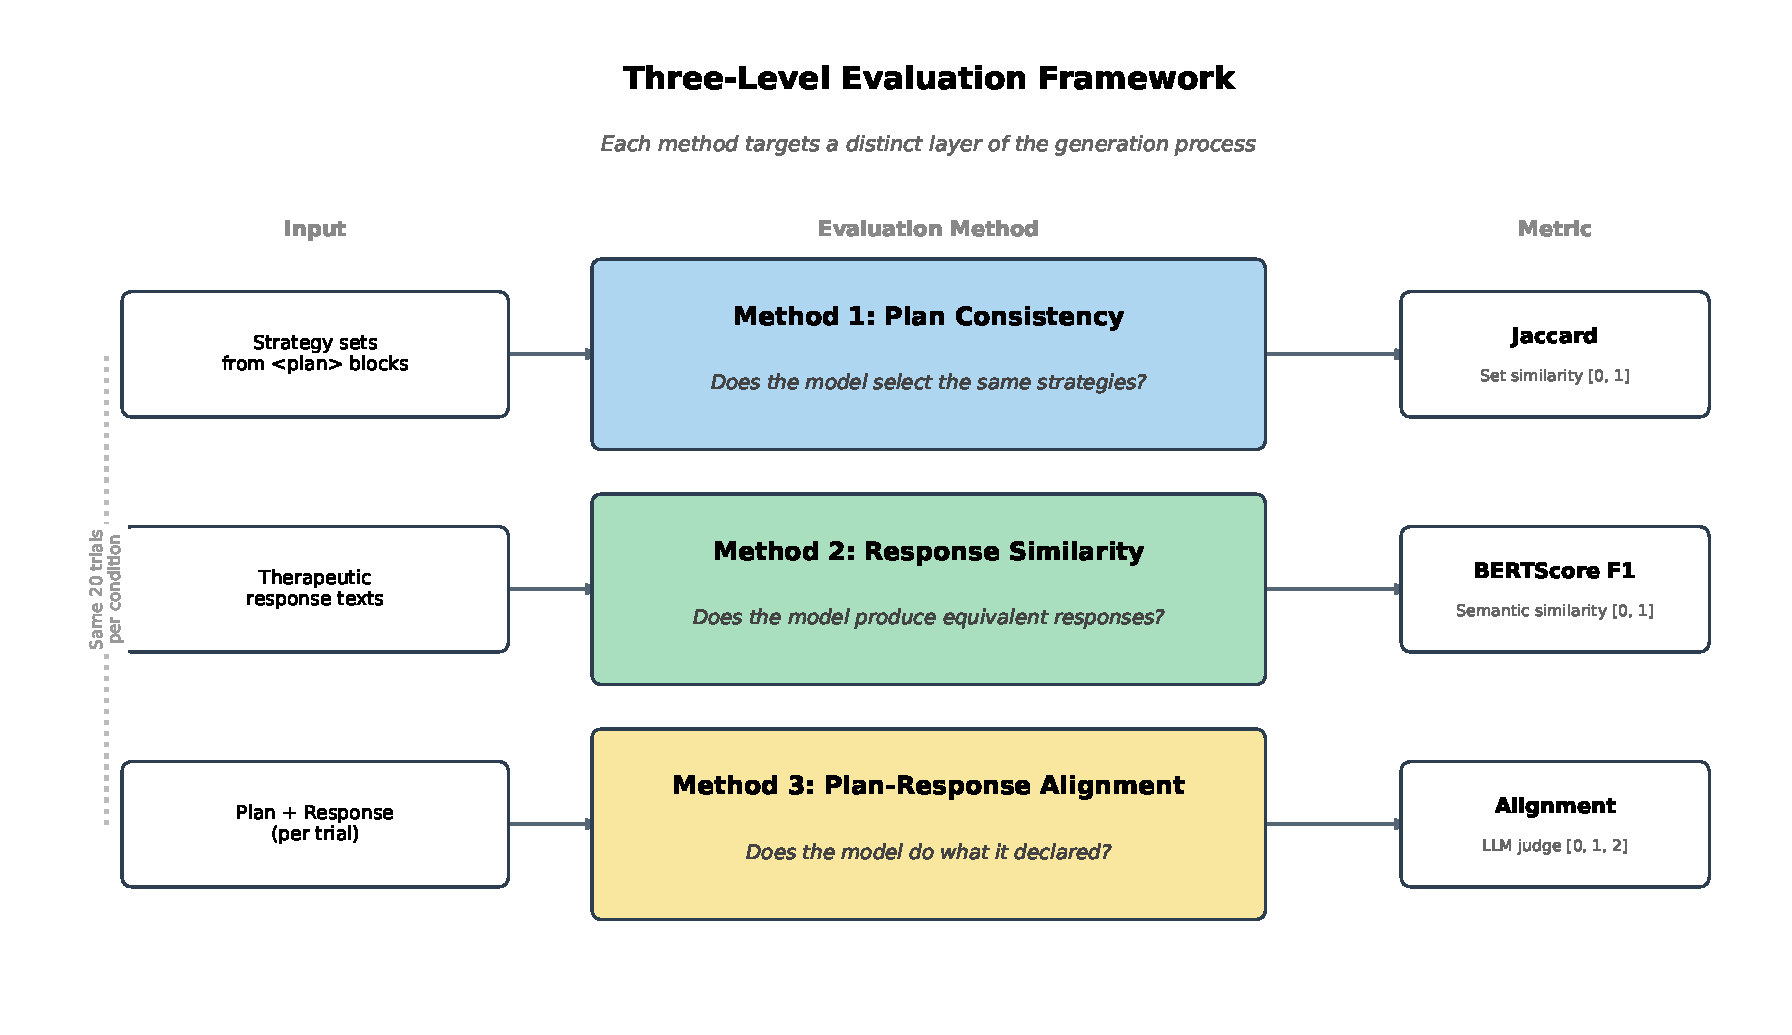
\includegraphics[width=1.2\textwidth]{figures/fig_3_2_measurement.pdf}}
  \caption{Three-level evaluation framework. Each method targets a
    distinct layer of the generation process: strategy selection (Jaccard),
    response wording (BERTScore), and plan-response coherence (LLM judge).}
  \label{fig:three-level}
\end{figure}

% previously: Cognitive Stability (Plan Consistency) -- renamed to avoid
% theoretically loaded term (supervisor feedback 2026-03-23)
\subsection{Method 1: Plan Consistency}
\label{sec:meth-m1}
% Pairwise Jaccard similarity over strategy sets from <plan> blocks
%   J(A,B) = |A n B| / |A u B|; mean over C(20,2) = 190 trial pairs
% Strategy extraction from <plan> blocks. Validity rate as upstream quality gate
%   -- malformed plans excluded
% Why Jaccard? Set similarity is appropriate for unordered strategy
%   combinations; insensitive to labelling artefacts
% Measures: do stochastic runs produce the same therapeutic decisions?
% [Example] 10 plan sets -> pairwise Jaccard matrix -> mean score;
%   one high- and one low-consistency condition shown

Method~1 measures whether the model selects the same therapeutic strategies
across independent trials. Strategy sets are extracted from the
\techil{<plan>} block of each trial output using the fixed taxonomy from
\autoref{tab:taxonomy}. Pairwise Jaccard similarity quantifies agreement
between strategy sets:

\begin{equation}
  J(A, B) = \frac{|A \cap B|}{|A \cup B|}
\end{equation}

The mean Jaccard score is computed over all $\binom{20}{2} = 190$ trial
pairs per condition. Jaccard is appropriate because strategy combinations
are unordered sets: a model that declares \emph{confrontation / cognitive
reframe} has made the same clinical decision as one that declares
\emph{cognitive reframe / confrontation}.

Because Jaccard operates on discrete sets of one to two items drawn from
six categories, it takes only a small number of distinct values:
$\{0, 0.33, 0.5, 0.67, 1.0\}$. All three metrics are reported with means
and standard deviations, aggregated across vignettes.

Plan validity rate serves as an upstream quality gate. A malformed
\techil{<plan>} block that cannot be parsed into valid strategy identifiers
is excluded from the Jaccard computation. The validity rate reports the
proportion of trials with parseable plans, indicating whether the model can
follow the structured output format at all.

% [Example] 10 plan sets, pairwise Jaccard matrix, mean score

% previously: Output Consistency (Semantic Stability) -- renamed for clarity
\subsection{Method 2: Response Similarity}
\label{sec:meth-m2}
% GROUNDING: builds on the metric landscape from Section 2.4
%
% Pairwise BERTScore F1 over response texts; mean over C(20,2) = 190 pairs
% Embedding model choice: DeBERTa-XLarge-MNLI (He et al., 2021)
%   Why this model?
%   - NLI fine-tuning aligns with semantic similarity over surface matching
%   - Highest WMT16 human correlation (r = 0.778) among available options
%   - Disentangled attention handles surface-form variation in therapeutic language
%     where valid paraphrasing is the norm
% Why not BLEU/ROUGE? Surface metrics penalise valid therapeutic paraphrasing
%   (established in 2.4) -- embedding similarity is the appropriate level
% Measures: do stochastic runs produce therapeutically equivalent responses?
% [Example] Two responses from the same condition -> token alignment
%   heatmap -> F1; one high- and one low-similarity pair

Method~2 measures whether the model produces semantically similar
responses across trials, independent of strategy declarations. Pairwise
BERTScore F1 is computed over response texts (with plan blocks excluded)
across the same 190 trial pairs. The embedding model is
\modelname{DeBERTa-XLarge-MNLI} \parencite{8MQC2H2V}, selected for its
high correlation with human similarity judgements as discussed in
\autoref{sec:bg-metrics}.

% [Example] Two responses from the same condition, alignment heatmap, F1

% previously: Plan-Response Coherence
\subsection{Method 3: Plan-Response Coherence}
% originally exploratory -- may restore label depending on results
\label{sec:meth-m3}
% GROUNDING: addresses the multi-level gap from Section 2.4
%   (no single metric captures strategic intent + semantic similarity)
%
% LLM judge: Gemini 3.1 Pro (Google AI Studio, T=1.0), cross-family with
%   all evaluation targets. Thinking mode aids judgment accuracy.
%   T=1.0 is the Gemini 3 default; Google warns against lowering it.
%   0 = absent, 1 = partial, 2 = implemented
% Why ternary? Borrowed from clinical fidelity literature (ENACT, NIH BCC,
%   introduced in 2.1); binary scoring loses partial implementation --
%   clinically meaningful
% Why LLM judge? Only approach capable of multi-strategy coherence with
%   a reasoning trace; NLI cross-encoders ceiling at F1 ~0.55 on this task
% Rejected alternatives: NLI cross-encoders (F1 ceiling ~0.55, task mismatch,
%   no reasoning trace)
% Mitigations for known judge biases (identified in 2.4):
%   cross-model judging, CoT justification, T=1.0, transparent rubric
% Labelled exploratory: judge reliability is itself an open question
% Validation: human annotation of a random subset (~50 trials) scoring the
%   same rubric. Cohen's kappa between human and judge as reliability estimate.
%   If kappa is low, Method 3 results carry the caveat explicitly.
% Measures: does the model's response implement its declared therapeutic plan?
% [Example] Judge input + output -- plan, response, ternary verdict with
%   CoT justification; partial and absent case shown

Method~3 measures whether the model's therapeutic response implements its
declared strategy. A separate \gls{llm} judge scores each declared strategy
on a ternary scale:

\begin{itemize}
  \item \textbf{0 (absent):} The strategy is not reflected in the response.
  \item \textbf{1 (partial):} The strategy is mentioned but not fully developed.
  \item \textbf{2 (implemented):} The strategy is clearly and substantively present.
\end{itemize}

This ternary scale follows the ENACT and NIH BCC fidelity frameworks
introduced in \autoref{sec:bg-irt}.

The judge model is \modelname{Gemini 3.1 Pro}, accessed through Google AI
Studio at $T = 1.0$, the Gemini~3 default. Lowering the temperature below
1.0 can cause looping or degraded output for Gemini~3 models
\parencite{W2RFM6E4}. \modelname{Gemini} is from a different model family
than all evaluation targets, preventing self-preference bias. Its thinking
mode supports structured reasoning about whether a response implements a
given strategy. The judge receives the strategy definitions, the declared
strategies, and the response text, and produces a score with justification
for each strategy. \modelname{Gemini~3~Pro} has been validated as a
reliable judge for content validity assessment in psychology
\parencite{XQDRY83T}.

Bias mitigations follow established recommendations
\parencite{LVLA9LZU}: cross-model judging, \gls{cot} justification, and
a transparent rubric anchoring scores to specific behavioural criteria.
\gls{nli} cross-encoders were considered but rejected after preliminary
testing showed an F1 ceiling of approximately 0.55 on this task.

Judge reliability is validated through human annotation of a stratified
random subset of 60 trials (covering all ten models), scoring the same
ternary rubric. Cohen's $\kappa$ between human and judge is $0.777$
(linear-weighted), indicating substantial agreement. Exact agreement is
89.2\%. All 13 disagreements go in one direction: the human annotator
scored higher than the judge, indicating a conservative rather than
lenient bias.

% Coherence ceiling finding moved to Discussion (sec:disc-framework-interpretation).

% [Example] Judge input/output -- plan, response, ternary verdict with CoT


\section{Model Selection}
\label{sec:meth-models}
% GROUNDING: regulatory framing established in 2.2
%
% EU data sovereignty as primary selection criterion -- self-hostability and EU data
%   residency are legal constraints in the reDreamAI deployment context
% All evaluation targets run in non-thinking mode for fair comparison.
%   Qwen 3.5 and Mistral Small 4 (hybrid-thinking) run with reasoning disabled.
%
% Primary subject: Mistral Large 3 (675B MoE, 41B active)
%   EU-sovereign, Apache 2.0, frontier-class
% EU-sovereign comparators: Mistral Small 4 (119B MoE), Mistral Small 3.2 (24B dense)
% Proprietary ceiling: GPT-5.4 and Sonnet 4.6 (non-thinking variants)
% Open-weight comparators across size classes and architectures
% Selection rationale: size-class diversity, dense vs MoE architecture,
%   provider diversity, EU sovereignty depth
% [FIG] Model selection table -- model, size, architecture, provider,
%   sovereignty status, role in study

\gls{eu} data sovereignty serves as the primary selection criterion for the
study's main subject. The deployment context (reDreamAI) requires a model
that can be self-hosted within \gls{eu} data residency boundaries
\parencite{2QMKF3RM}. All evaluation targets run in non-thinking mode for
fair comparison.

The primary subject is \modelname{Mistral Large~3} (675B \gls{moe}, 41B
active parameters, Apache~2.0), the \gls{eu}-sovereign flagship and the
model that reDreamAI would deploy in production. Two additional Mistral
models complete the family comparison: \modelname{Mistral Small~4}
(119B \gls{moe}, 6.5B active) is the newest and most parameter-efficient
\gls{moe} in the set, and \modelname{Mistral Small 3.2} (24B dense)
serves as a dense predecessor baseline.

Two proprietary models provide a ceiling reference.
\modelname{GPT-5.4} (non-thinking variant) is the strongest proprietary
model without thinking overhead. \modelname{Claude Sonnet~4.6} adds a second proprietary reference point
from a different vendor.

Five open-weight comparators span three size classes and two
architectures. \autoref{tab:models} lists all ten models with their
selection rationale.

\begin{table}[t]
  \centering
  \caption{Evaluation targets. All models run in non-thinking mode via OpenRouter.}
  \label{tab:models}
  \begin{tabularx}{\textwidth}{llrX}
    \toprule
    Group & Model & Size & Selection rationale \\
    \midrule
    \multicolumn{4}{l}{\emph{EU-sovereign (Mistral, Apache~2.0)}} \\
    Primary   & \modelname{Mistral Large 3}   & 675B \gls{moe} (41B active)   & \gls{eu}-sovereign flagship. Production deployment candidate \\
    EU        & \modelname{Mistral Small 4}   & 119B \gls{moe} (6.5B active)  & Newest Mistral. Fewest active parameters of any \gls{moe} in set \\
    EU        & \modelname{Mistral Small 3.2} & 24B dense                      & Dense predecessor to Small~4 \\
    \addlinespace
    \multicolumn{4}{l}{\emph{Open-weight comparators}} \\
    \gls{moe} & \modelname{Qwen 3.5 397B}    & 397B \gls{moe} (17B active)   & Large \gls{moe} comparator to Mistral Large~3 \\
    \gls{moe} & \modelname{Qwen 3.5 122B}    & 122B \gls{moe} (10B active)   & Peer \gls{moe} comparator to Mistral Small~4 \\
    Dense     & \modelname{Qwen 3.5 27B}     & 27B dense                      & Same size class as Mistral Small 3.2 \\
    Dense     & \modelname{OLMo 3.1 32B}     & 32B dense                      & Fully open (weights, data, code). Best provenance \\
    Dense     & \modelname{Llama 3.3 70B}    & 70B dense                      & Continuity with prior efficacy study \\
    \addlinespace
    \multicolumn{4}{l}{\emph{Proprietary ceiling}} \\
    Ceiling   & \modelname{Claude Sonnet 4.6} & Proprietary                   & Latest Claude model, known for natural conversational style \\
    Ceiling   & \modelname{GPT-5.4}           & Proprietary                   & Strongest non-thinking proprietary model \\
    \bottomrule
  \end{tabularx}
\end{table}

The selection provides size-class diversity (24B--675B), architectural
diversity (dense \vs \gls{moe}), and provider diversity across five
vendors. \modelname{Qwen 3.5} and \modelname{Mistral Small~4} are
hybrid-thinking models that support optional reasoning. To maintain fair
comparison, reasoning is disabled for all evaluation targets. All
OpenRouter calls specify the model vendor as the inference provider,
ensuring that each model runs on the same backend across all trials.

Including three Qwen scales (27B, 122B, 397B) enables within-family
scaling analysis.\footnote{\modelname{DeepSeek V3.2} was originally
considered for this slot but dropped because its internal temperature
scaling would have complicated cross-model comparison.}


\section{Experimental Conditions}
\label{sec:meth-conditions}
% Full factorial: 6 vignettes x 5 temperatures x 20 trials x 10 models
% Temperature sweep: 0.0, 0.075, 0.15, 0.3, 0.6
%   0.0: deterministic baseline (greedy decoding)
%   0.15: Mistral vendor default
%   0.6: Qwen/Llama/OLMo vendor default, close to GPT/Sonnet 0.7
%   0.075: added post-hoc when Mistral peaked between 0.0 and 0.15
% [FIG] Condition matrix -- factorial design as a grid; total run count labelled

The experiment follows a full factorial design:

\begin{table}[t]
  \centering
  \caption{Experimental conditions. Total: $6 \times 5 \times 20 = 600$ trials per model, 6{,}000 across all ten models.}
  \label{tab:conditions}
  \begin{tabular}{ll}
    \toprule
    Dimension & Values \\
    \midrule
    Vignettes    & anxious, avoidant, cooperative, resistant, skeptic, trauma \\
    Trials       & 20 per condition \\
    Temperatures & $T \in \{0.0,\; 0.075,\; 0.15,\; 0.3,\; 0.6\}$ \\
    Models       & 10 evaluation targets (\autoref{tab:models}) \\
    \bottomrule
  \end{tabular}
\end{table}

Rather than testing only two temperature conditions, the experiment uses a
five-point temperature sweep that spans from deterministic decoding to the
vendor-recommended defaults. The scale is anchored at three points
motivated by vendor documentation:

\begin{description}
  \item[$T = 0.0$] (greedy decoding) serves as a deterministic upper
    bound on stability. Even at $T = 0.0$, GPU parallelisation introduces
    floating-point non-determinism \parencite{HITR7PL4}, so the
    twenty-trial design captures residual variance directly
    \parencite{WA4QD3UE}.
  \item[$T = 0.15$] is the recommended temperature for Mistral models.
    \modelname{Mistral Small 3.2} sets this value explicitly in its
    HuggingFace generation configuration. \modelname{Mistral Large 3}
    and \modelname{Mistral Small 4} lack a generation configuration
    default. Their model cards recommend temperatures below 0.1 for
    production use, while code examples on the same cards use
    $T = 0.15$. Because no authoritative single default exists for these
    two models, 0.15 was chosen to match the verified
    \modelname{Small 3.2} value and the vendor code examples.
  \item[$T = 0.6$] is the default for \modelname{Qwen 3.5} and
    \modelname{OLMo~3.1}, also close to the standard Llama chat range
    (0.6--0.7) and the proprietary defaults (\modelname{GPT-5.4} and
    \modelname{Sonnet~4.6} default to $T = 0.7$).
    % Sources: Qwen 3.5 generation_config.json [VERIFIED],
    %   OLMo 3.1 generation_config.json [VERIFIED],
    %   Llama 3.3 generation_config.json via unsloth mirror + meta-llama/llama3 reference impl [VERIFIED]
    %   GPT-5.4 -- reasoning model, does not support temperature parameter
    %   Sonnet 4.6 -- Anthropic API docs, default 1.0, 0.7 as midpoint [VERIFIED]
\end{description}

The intermediate points $T = 0.075$ and $T = 0.3$ fill the gap between
Mistral's low default and the Qwen/Llama range. $T = 0.075$ was added
after an initial four-point run revealed that several models peak in
consistency between $T = 0.0$ and $T = 0.15$, suggesting that a small
amount of sampling variance can be beneficial (discussed in
\autoref{sec:res-plan-consistency}).


\section{Statistical Analysis}
\label{sec:meth-stats}
% Descriptive statistics: medians/IQR for Jaccard (ordinal), means/SD for
%   BERTScore and alignment, confidence intervals across 190 trial pairs
% Spearman rank correlations for cross-method analysis (\autoref{sec:res-cross})
%   and per-model temperature effects
%   Why Spearman: rank-based, robust to non-normal distributions from
%   bounded similarity scores
% Kruskal-Wallis for model and vignette group differences
% No fixed threshold for ``stable enough.'' Results are interpreted comparatively
%   (model vs model, across temperature sweep) rather than against an absolute cutoff.
%   Clinical significance thresholds for LLM stability do not yet exist.

The analysis is primarily descriptive. For each model and temperature
condition, central tendency and dispersion are reported for all three
evaluation metrics, aggregated across vignettes.
All three metrics are reported with means and standard deviations.

Spearman rank correlations serve two purposes. First, per-model
correlations between Jaccard and temperature quantify the temperature
sensitivity of each model across the five-point sweep. Second,
cross-method correlations (Method~1 \vs Method~2, Method~1 \vs Method~3,
Method~2 \vs Method~3) assess whether the three evaluation layers capture
redundant or independent information. If they diverge, the clinical
implications differ: high plan consistency with low response similarity
indicates stable strategy selections but variable execution, while the
reverse indicates different strategies producing similar surface outputs.
Spearman rather than Pearson is used because Jaccard takes only a small
set of discrete values and BERTScore distributions may be non-normal.

Kruskal-Wallis tests assess whether models and vignettes differ
significantly on each metric. These are exploratory rather than
confirmatory: the study is designed to describe stability patterns, not to
test a preregistered hypothesis.

No fixed threshold defines ``stable enough.'' Clinical significance
thresholds for \gls{llm} stability do not yet exist in the literature.
Results are interpreted comparatively: model against model, across the
temperature sweep. The random Jaccard baseline (expected value for random
2-of-6 selections, approximately 0.2) provides a lower reference point.
